%%%%%%%%%%%%%%%%%%%%%%%%%%%%%%%%%%%%%%%%%%%%%%%%%%%%%%%%%%%%%%%%%%%%%%%%%%%%%%%
%                     Отчёт по лабораторной работе №5
%
% Дисциплина: Теория вероятностей и Математическая статистика
%                     
% Название:   Двумерная случайная величина: Выборочные кэффициенты корреляции, 
%             эллипсы рассеивания
%
% Выполнил:   Михаил Маляренко
%
% Дата:       6 Дек. 2020
%
%%%%%%%%%%%%%%%%%%%%%%%%%%%%%%%%%%%%%%%%%%%%%%%%%%%%%%%%%%%%%%%%%%%%%%%%%%%%%%%

% HEADER BEGIN 
\documentclass[12pt]{article}
\usepackage[utf8]{inputenc}
\usepackage[russian]{babel}
\usepackage{pscyr}
\usepackage[T2A]{fontenc}
\usepackage{geometry}
\usepackage{graphicx}
\usepackage{multirow}
\usepackage{hhline}
\usepackage{amsmath}
\usepackage{amssymb}
\usepackage{hyperref}
\usepackage{xcolor}

\geometry {	
	a4paper, 
	left   = 20mm, 
	right  = 20mm, 
	top    = 20mm, 
	bottom = 20mm
}

\definecolor{urlcolor}{HTML}{2484BC} 
\definecolor{linkcolor}{HTML}{000000}

\graphicspath{{resource/}}
% HEADER END

% DIFINES BEGIN
\newcommand{\lskip}{\hfill\break}
% DEFINES END

\begin{document}

\begin{titlepage}
	\begin{center}
		\hfill \break
		{\textbf{Санкт-Петербургский политехнический университет Петра Великого}}\\
		\hfill \break
		\textbf{Институт прикладной математики и механики}\\
		 \hfill \break
		\textbf{Кафедра <<Телематика (при ЦНИИ РТК)>>}\\
		\vfill
		\large{\bfseries Отчет по лабораторной работе}\\
		\hfill \break
		\hfill \break
		\hfill \break
		\hfill \break
        \normalsize{\bfseries Двумерная случайная величина:
        
        выборочные коэффициенты корреляции и эллипсы рассеивания}\\
        \hfill \break
		По дисциплине <<Теория вероятностей и Математическая статистика>>\\
		\hfill \break
		\hfill \break
	\end{center}
 
	\normalsize
	{ 
		\begin{tabular}{lp{2cm}cr}
			Выполнил &&&\\
			Студент гр. 3630201/80101&&\underline{\hspace{1.5cm}}& М. Д. Маляренко\\\\
			Руководитель&&&\\ 
			к.ф.-м.н., доцент && \underline{\hspace{1.5cm}}& А. Н. Баженов \\\\
			&&&<<\underline{\phantom{333}}>>\underline{\phantom{сентября000}}
			2020г.
		\end{tabular}
	}
\vfill

\begin{center} Санкт-Петербург \\2020 \end{center}
\end{titlepage}

\newpage

\setcounter{page}{2}

\begin{flushleft}

\setlength{\parindent}{1cm}

% TABLE OF CONTENTS
\tableofcontents

\newpage

% LIST OF FIGURES
\listoffigures

\newpage

% LIST OF TABLES
\listoftables

\newpage

\section{Постановка задачи}

    Сгенерировать двумерные выборки размерами 20, 60, 100 для нормального двумерного распределения $N(x, y, 0, 0, 1, 1, \rho)$ с коэффициентами корреляции $\rho = 0, \; 0.5, \; 0.9$. Изобразить сгенерированные точки на плоскости и нарисовать эллипс рассеивания. Каждую выборку сгенерировать 1000 раз и вычислить среднее значение, среднее значение квадрата и дисперсию

    \begin{enumerate}
        \item Выборочных коэффициентов корреляции Пирсона
        \item Выборочных коэффициентов корреляции Спирмена
        \item Выборочных квадратных коэффициентов
    \end{enumerate}

    Повторить все вычисления для смеси нормальных распределений:

    \begin{equation}
        f(x,y) = 0.9N(x, y, 0, 0, 1, 1, 0.9) + 0.1N(x, y, 0, 0, 10, 10, -0.9)
        \label{normal_mix}
    \end{equation}

\newpage

\section{Теория}

    \subsection{Двумерное нормальное распределение}

    Двумерная случайная величина $(X, Y)$ называется распределённой нормально (или просто нормальной), если её плотность вероятности определена формулой

    \begin{multline}
            N(x, y, \overline{x}, \overline{y}, \sigma_x, \sigma_y, \rho) = \frac{1}{2\pi\sigma_x\sigma_y\sqrt{1 - \rho^2}} \times\\
            \times \exp\left\{ -\frac{1}{2(1 - \rho^2)} \left[ \frac{(x - \overline{x})^2}{\sigma_x^2} - 2\rho\frac{(x - \overline{x})(y - \overline{y})}{\sigma_x\sigma_y} + \frac{(y - \overline{y})^2}{\sigma_y^2}\right] \right\}
        \label{normal2}
    \end{multline}

    Компоненты $X, Y$ двумерной нормальной случайной величины также распределены нормально с математическими ожиданиями $\overline{x}, \overline{y}$ и средними квадратическими отклонениями $\sigma_x, \sigma_y$ соответственно \cite{theory1}. Параметр $\rho$ называется коэффициентом корреляции.

    \subsection{Корреляционный момент (ковариация) и коэффициент корреляции}
        Корреляционный момент, иначе ковариация, двух случайных величин $X$ и $Y$:
        \begin{equation}
            K = cov(X, Y) = M\left[(X-\overline{x})(Y-\overline{y})\right]
        \end{equation}

        \noindentКоэффициент корреляции $\rho$ двух случайных величин $X$ и $Y$:
        \begin{equation}
            \rho = \frac{K}{\sigma_x\sigma_y}
        \end{equation}    

    \subsection{Выборочные коэффициенты корреляции}
        \subsubsection{Выборочный коэффициент корреляции Пирсона}
            Выборочный коэффициент корреляции Пирсона:

            \begin{equation}
                r = \frac{\frac{1}{n} \sum (x_i - \overline{x})(y_i - \overline{y})}{\sqrt{\frac{1}{n} \sum (x_i - \overline{x})^2 \frac{1}{n} \sum (y_i - \overline{y})^2}} = \frac{K}{s_Xs_Y},
            \label{pirse}
            \end{equation}

            где $K, s_X^2, s_Y^2$ -- выборочные ковариация и дисперсии с.в. $X$ и $Y$.

        \subsubsection{Выборочный коэффициент ранговой корреляции Спирмена}
        Обозначим ранги, соответствующие значениям переменной $X$, через $u$, а ранги, соответствующие значениям переменной $Y$, — через $v$.

        Выборочный коэффициент ранговой корреляции Спирмена :
        \begin{equation}
            r_S = \frac{\frac{1}{n} \sum (u_i - \overline{u})(v_i - \overline{v})}{\sqrt{\frac{1}{n} \sum (u_i - \overline{u})^2 \frac{1}{n} \sum (v_i - \overline{v})^2}},
            \label{spirmen}
        \end{equation} 
        где $\overline{u} = \overline{v} = \frac{1 + 2 + ... + n}{n} = \frac{n+1}{2}$ -- среднее значение рангов.

        \subsubsection{Выборочный квадрантный коэффициент корреляции}
            Выборочный квадрантный коэффициент корреляции
            \begin{equation}
                r_Q = \frac{(n_1+n_3) - (n_2 + n_4)}{n}, 
                \label{square}
            \end{equation} 
            где $n_1, n_2, n_3, n_4$ -- количества точек с координатами $(x_i, y_i)$, попавшими соответственно в I, II, III и IV квадранты декартовой системы с осями $x' = x - med \; x, y' = y - med \; y$ и с центром в точке с координатами $(med \; x, med \; y)$.

    \subsection{Эллипсы рассеивания}

    Уравнение проекции эллипса рассеивания на плоскость $xOy$:

    \begin{equation}
        \frac{(x-\overline{x})^2}{\sigma_x^2} - 2\rho\frac{(x-\overline{x})(y-\overline{y})}{\sigma_x\sigma_y} + \frac{(y-\overline{y})^2}{\sigma_y^2} = const.
        \label{ellipse}
    \end{equation}

    Центр эллипса (\ref{ellipse}) находится в точке с координатами $(\overline{x}, \overline{y})$; оси симметрии эллипса составляют с осью $Ox$ углы, определяемые уравнением

    \begin{equation}
        tg 2\alpha = \frac{2\rho\sigma_x\sigma_y}{\sigma_x^2 - \sigma_y^2}.
    \end{equation} 

\newpage

\section{Реализация}

    Расчёты и построение графиков производились в среде аналитических вычислений Maxima. Для построения выборок двумерного нормального распределения, вычисления выборочных коэффициентов корреляции Пирса, Спирмена и квадратного выборочного коэффициента корреляции были написаны функции соответственно \texttt{random2\_normal}, \texttt{r}, \texttt{r\_S} и \texttt{r\_Q}. 
    
    Смесь двумерных нормальных распределений происходила по следующей схеме: генерировалась выборка равномерно распределённых непрерывных случайных чисел в диапазоне $[0, 1]$. В цикле по элементам этой выборки происходила генерация двумерного нормального распределения с нужными параметрами. В случае, если элемент выборки равномерного распределения $< 0.1$, то генерировалась пара чисел двумерного нормального распределения с весовым коэффициентом $0.1$, в обратном случае -- с весовым коэффициентом $0.9$ (см. (\ref{normal_mix})). 
    
    Для построения графиков использовалась интегрированная в среду утилита gnuplot. Полный текст скрипта для среды Maxima представлен в репозитории GitHub.

\newpage

\section{Результаты}

    \subsection{Выборочные коэффициенты корреляции}

        В Таблице \ref{table_normal} представлены выборочные коэффициенты корреляции Прирса (\ref{pirse}), Спирмена (\ref{spirmen}) и квадратный коэффициент корреляции (\ref{square}) для выборок размера 20, 60 и 100 элементов двумерного нормального распределения $N(x, y, 0, 0, 1, 1, \rho)$ с коэффициентами корреляции $\rho = 0, \; 0.5, \; 0.9$.

        \begin{table}[h]
            \begin{center}
                \caption{Выборочные коэффициенты корреляции для двумерного нормального распределения}
                \begin{tabular}{||c|c||*{3}{c|}|*{3}{c|}|*{3}{c|}|} \hhline{~~|t:===:t:===:t:===:t|}
                \multicolumn{2}{c||}{} & \multicolumn{3}{c||}{$r$} & \multicolumn{3}{c||}{$r_Q$} & \multicolumn{3}{c||}{$r_S$}\\ 
                \hhline{~~||---||---||---||}
                \multicolumn{2}{c||}{} & $E(z)$ & $E(z^2)$ & $D(z)$ & $E(z)$ & $E(z^2)$ & $D(z)$ & $E(z)$ & $E(z^2)$ & $D(z)$\\ 
                \hhline{|t:==::===::===::===:|}

                \multirow{3}*{$\rho = 0$} & $N = 20$ & $0.0$ & $0.05$ & $0.05$ & $0.0$ & $0.05$ & $0.05$ & $0.0$ & $0.05$ & $0.05$\\ 
                \hhline{~|-||---||---||---||}
                                            & $N = 60$ & $0.0$ & $0.02$ & $0.02$ & $0.0$ & $0.02$ & $0.02$ & $0.0$ & $0.02$ & $0.02$\\ 
                \hhline{~|-||---||---||---||}
                                            & $N = 100$ & $0.0$ & $0.01$ & $0.01$ & $0.0$ & $0.01$ & $0.01$ & $0.0$ & $0.01$ & $0.01$\\ 
                \hhline{|:=:=::===::===::===:|}

                \multirow{3}*{$\rho = 0.5$} & $N = 20$ & $0.5$ & $0.27$ & $0.03$ & $0.3$ & $0.16$ & $0.05$ & $0.5$ & $0.25$ & $0.03$\\
                \hhline{~|-||---||---||---||}
                                            & $N = 60$ & $0.5$ & $0.25$ & $0.01$ & $0.33$ & $0.12$ & $0.01$ & $0.5$ & $0.24$ & $0.01$\\
                \hhline{~|-||---||---||---||}
                                            & $N = 100$ & $0.49$ & $0.253$ & $0.006$ & $0.33$ & $0.120$ & $0.009$ & $0.48$ & $0.234$ & $0.006$\\ 
                \hhline{|:=:=::===::===::===:|}

                \multirow{3}*{$\rho = 0.9$} & $N = 20$ & $0.89$ & $0.800$ & $0.003$ & $0.68$ & $0.50$ & $0.03$ & $0.87$ & $0.749$ & $0.005$\\
                \hhline{~|-||---||---||---||}
                                            & $N = 60$ & $0.89$ & $0.809$ & $0.007$ & $0.70$ & $0.505$ & $0.009$ & $0.88$ & $0.782$ & $0.001$\\
                \hhline{~|-||---||---||---||}
                                            & $N = 100$ & $0.90$ & $0.806$ & $0.004$ & $0.71$ & $0.506$ & $0.005$ & $0.88$ & $0.7837$ & $0.0007$\\
                \hhline{|b:=:=:b:===:b:===:b:===:b|}
                \end{tabular}
            \label{table_normal}
            \end{center}
        \end{table}

        В Таблице \ref{table_mix_normal} представлены выборочные коэффициенты корреляции Пирса, Спирмена и квадратный коэффициент корреляции для выборок смеси двумерных нормальных распределений (\ref{normal_mix}) размера 20, 60 и 100 элементов.

        \begin{table}[h]
            \begin{center}
                \caption{Выборочные коэффициенты корреляции для смеси двумерных нормальных распределений}
                \begin{tabular}{||c||*{3}{c|}|*{3}{c|}|*{3}{c|}|} \hhline{~|t:===:t:===:t:===:t|}
                \multicolumn{1}{c||}{} & \multicolumn{3}{c||}{$r$} & \multicolumn{3}{c||}{$r_Q$} & \multicolumn{3}{c||}{$r_S$}\\ 
                \hhline{~||---||---||---||}
                \multicolumn{1}{c||}{} & $E(z)$ & $E(z^2)$ & $D(z)$ & $E(z)$ & $E(z^2)$ & $D(z)$ & $E(z)$ & $E(z^2)$ & $D(z)$\\ 
                \hhline{|t:=::===::===::===:|}

                $N = 20$ & $-0.3$ & $0.5$ & $0.4$ & $0.5$ & $0.32$ & $0.04$ & $0.5$ & $0.29$ & $0.08$\\
                \hhline{||-||---||---||---||}
                $N = 60$ & $-0.6$ & $0.49$ & $0.09$ & $0.6$ & $0.34$ & $0.01$ & $0.5$ & $0.26$ & $0.03$\\
                \hhline{||-||---||---||---||}
                $N = 100$ & $-0.7$ & $0.52$ & $0.03$ & $0.56$ & $0.318$ & $0.007$ & $0.5$ & $0.24$ & $0.02$\\
                \hhline{|b:=:b:===:b:===:b:===:b|}
                \end{tabular}
            \label{table_mix_normal}
            \end{center}
        \end{table}

    \subsection{Эллипсы рассеивания}

    На Рис. \ref{rho_0} - \ref{rho_09} представлены графики выборок размера 20, 60 и 100 двумерного нормального распределения $N(x, y, 0, 0, 1, 1, \rho)$ с коэффициентом корреляции $\rho = 0, \; 0.5, \; 0.9$, а также теоретические эллипсы рассеивания, рассчитанными по формуле (\ref{ellipse}), где за константу из правой части уравнения взято число $(2.5\sigma_x)^2 = (2.5\sigma_y)^2 = (2.5)^2$

    \newpage

        \begin{figure}[h]
            \begin{minipage}[h]{0.325\linewidth}
                \center{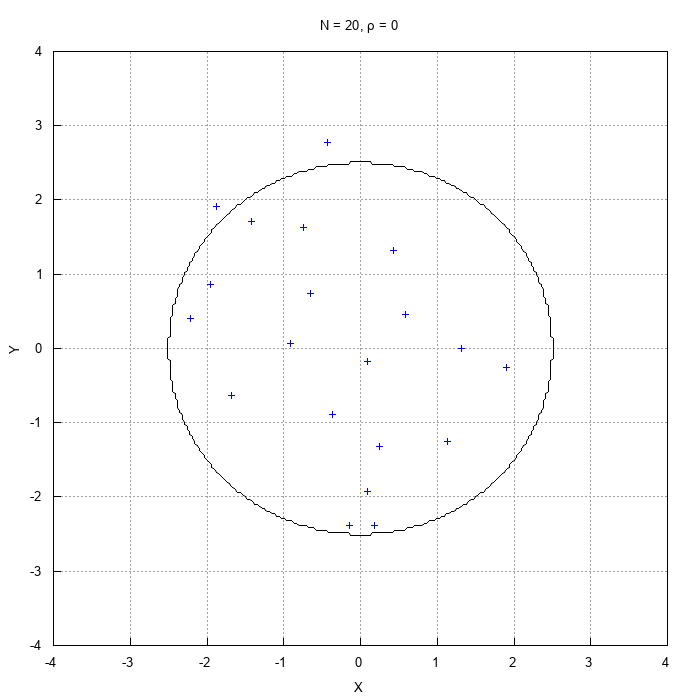
\includegraphics[width=1\linewidth]{N20R0.png}}
            \end{minipage}
            \begin{minipage}[h]{0.325\linewidth}
                \center{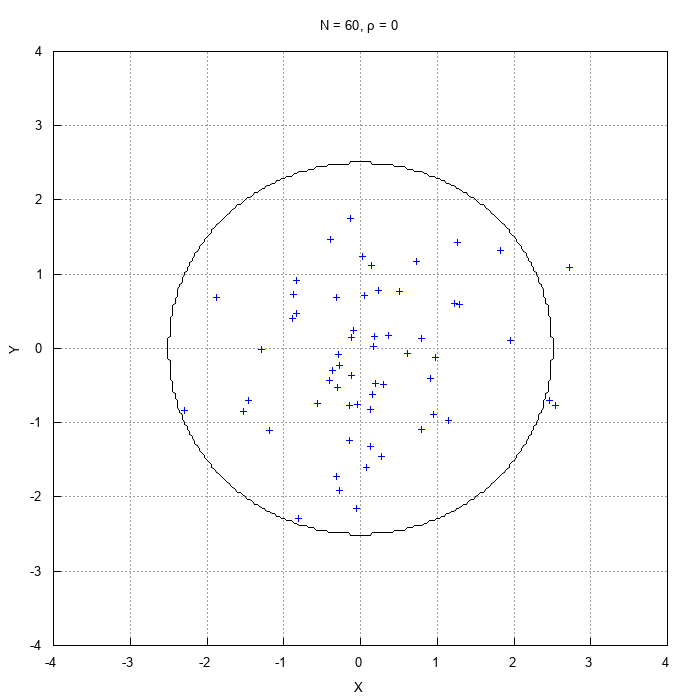
\includegraphics[width=1\linewidth]{N60R0.png}}
            \end{minipage}
            \begin{minipage}[h]{0.325\linewidth}
                \center{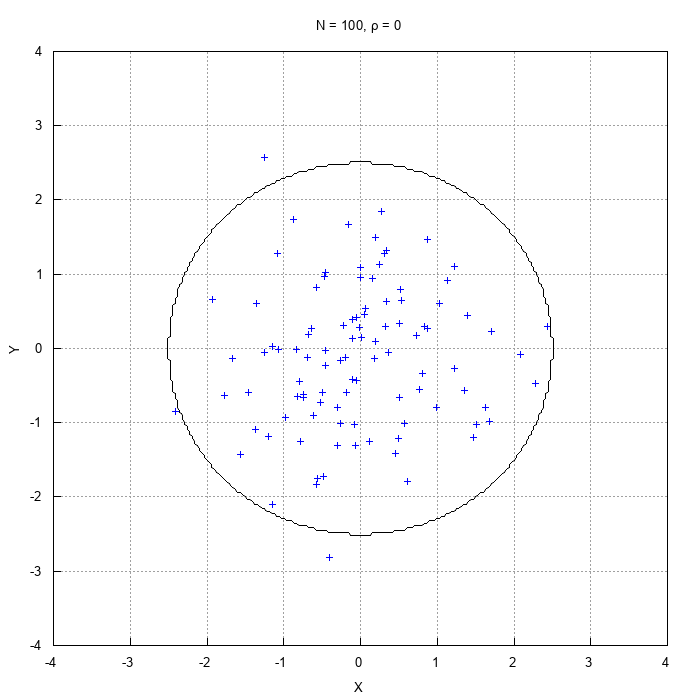
\includegraphics[width=1\linewidth]{N100R0.png}}
            \end{minipage}
            \caption{Эллипсы рассеивания для выборок нормального распределения с $\rho = 0$}
            \label{rho_0}
            \end{figure}

            \begin{figure}[h]
            \begin{minipage}[h]{0.325\linewidth}
                \center{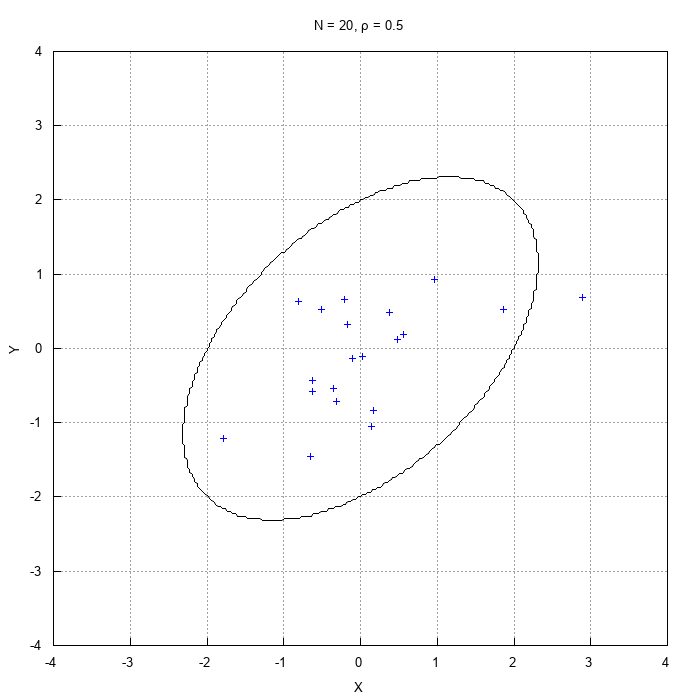
\includegraphics[width=1\linewidth]{N20R05.png}}
            \end{minipage}
            \begin{minipage}[h]{0.325\linewidth}
                \center{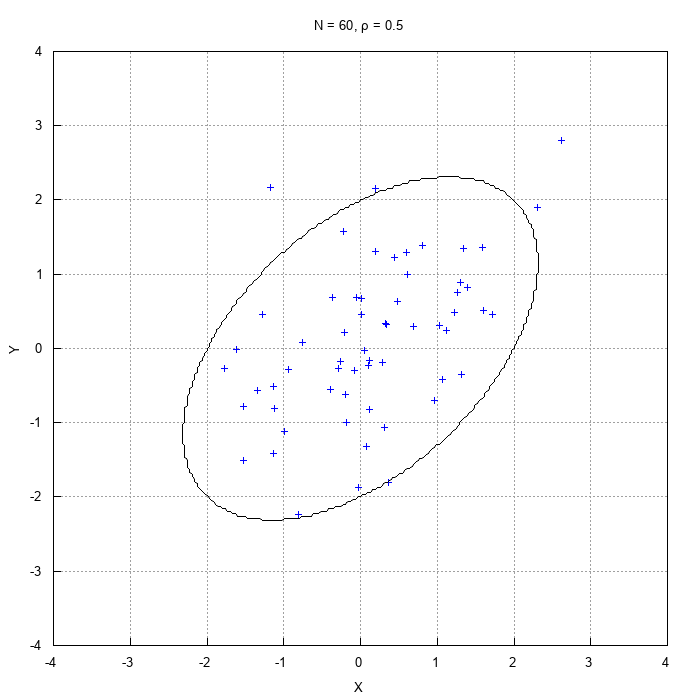
\includegraphics[width=1\linewidth]{N60R05.png}}
            \end{minipage}
            \begin{minipage}[h]{0.325\linewidth}
                \center{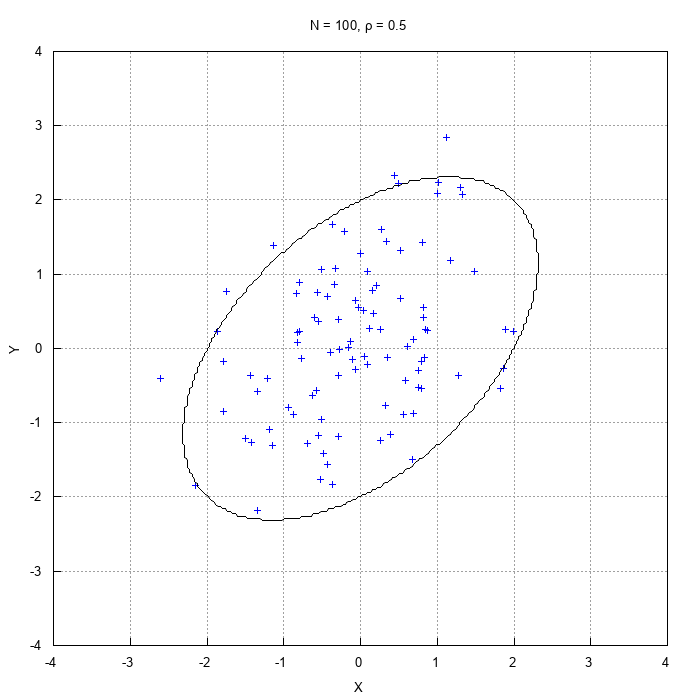
\includegraphics[width=1\linewidth]{N100R05.png}}
            \end{minipage}
            \caption{Эллипсы рассеивания для выборок нормального распределения с $\rho = 0.5$}
            \label{rho_05}
            \end{figure}

            \begin{figure}[h!]
            \begin{minipage}[h]{0.325\linewidth}
                \center{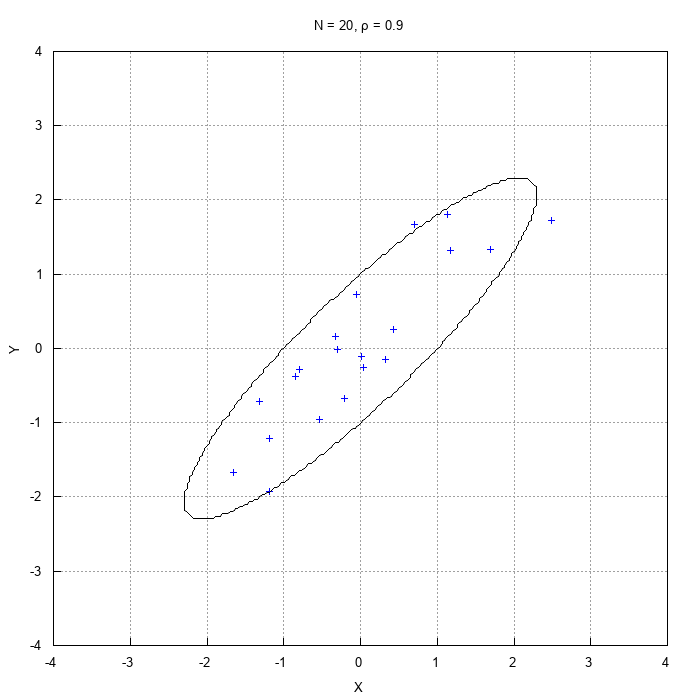
\includegraphics[width=1\linewidth]{N20R09.png}}
            \end{minipage}
            \begin{minipage}[h]{0.325\linewidth}
                \center{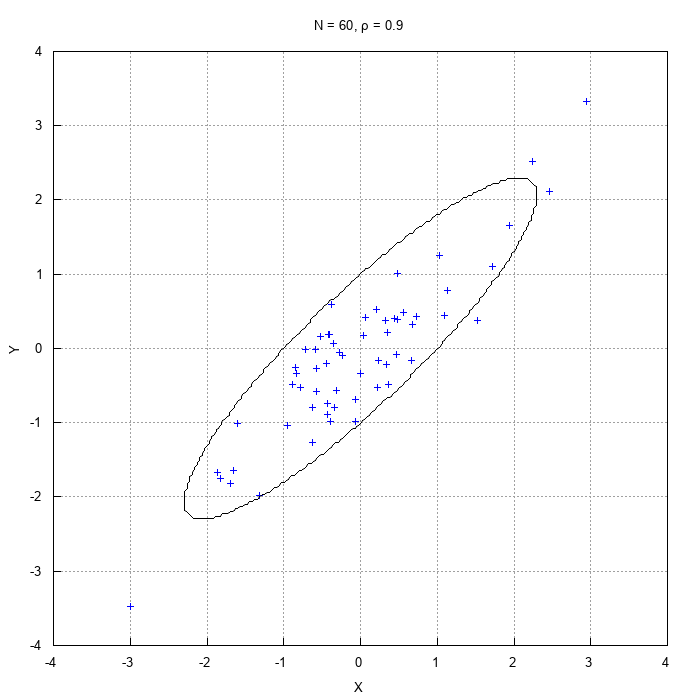
\includegraphics[width=1\linewidth]{N60R09.png}}
            \end{minipage}
            \begin{minipage}[h]{0.325\linewidth}
                \center{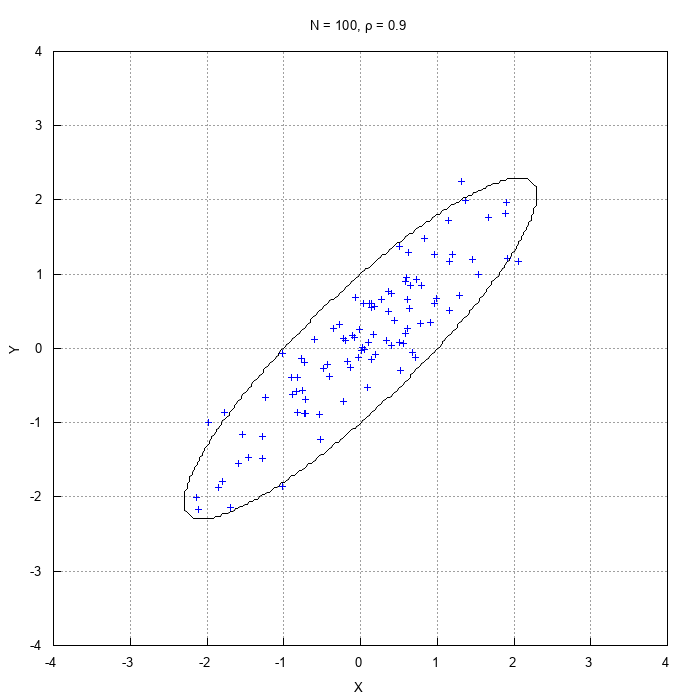
\includegraphics[width=1\linewidth]{N100R09.png}}
            \end{minipage}
            \caption{Эллипсы рассеивания для выборок нормального распределения с $\rho = 0.9$}
            \label{rho_09}
        \end{figure}

\newpage

\section*{Заключение}
\addcontentsline{toc}{section}{Заключение}

        В результате выполнения лабораторной работы были построены выборки двумерного нормального распределения с коэффициентами корреляции $\rho = 0, \; 0.5, \; 0.9$ и для смеси нормальных распределений. По оценкам выборочных коэффициентов корреляции можно сказать, что квадратный выборочный коэффициент имеет наибольшее отклонение от теоретического коэффициента корреляции, с увеличением мощности выборки все выборочные коэффициенты корреляции стремятся к своему теоретическому значению.

        По графикам двумерного нормального распределения видно, что чем больше коэффициент корреляции, тем более узкий эллипс рассеивания, в пределе при модуле коэффициента корреляции равном единице эллипс вырождается в прямую.

\newpage

\addcontentsline{toc}{section}{Список литературы}

\begin{thebibliography}{9}

        \bibitem{theory1}
        Теоретическое приложение к лабораторным работам №5-8 по дисциплине «Математическая статистика». -- СПб.: СПбПУ, 2020. -- 19 c
	
\end{thebibliography}

\newpage

\section*{Приложение А. Репозиторий с исходным кодом}
\addcontentsline{toc}{section}{Приложение А. Репозиторий с исходным кодом}

Исходный код скрипта для среды аналитических вычислений Maxima находится в репозитории GitHub -- URL \url{https://github.com/malyarenko-md/TeorVer}

\end{flushleft}

\end{document}